\chapter{Properties of Single-Wall Carbon Nanotubes}

\section{Introduction}
{\color{red}UNFINISHED} Carbon nanotubes are 1-D structures meaning that electrons are confined in a single dimension. They exist in terms of many chiralities, some are semiconducting and others are metallic \cite{soavi2016ultrafast}. Interesting because they let us explore the physics of 1-D structures. Due to the higher degree of confinement with respect to convention 3-D structures, different phenomena may occur.



\section{Carbon Nanotube Chiralities}

{\color{red}UNFINISHED} Carbon nanotubes are basically rolled up graphene sheets. Countless ways of rolling up a graphene sheet into cylindrical structures. Hence, nanotubes described using so-called chiral vectors. Species of carbon nanotubes are denoted using a set of indices ($m$,$n$). These integers $m$ and $n$ define the chiral vector $\vec{C_h }$ expressed as 
\begin{equation}
	\vec{C_h} = n \bm{\vec{a_1}} + m \bm{\vec{a_2}}
\end{equation}

where $\vec{a_1}$ and $\vec{a_2}$ represent the basis vectors of the 2D graphene sheet as shown in Figure \ref{fig:chiral_vectors} \cite{nanot2012optoelectronic}. In general, (n,n) carbon nanotubes constitute the set of all metallic nanotubes \cite{nanot2012optoelectronic}. All (n,m) nanotubes where $n-m = 3j$ ($j > 0$) comprise a set of small-gap ($\sim1 - 100$ meV) semiconductors \cite{nanot2012optoelectronic}. The remaining nanotubes outside of these two categories include medium-gap semiconductors ($\sim0.5 - 1$ eV) \cite{nanot2012optoelectronic}.

\begin{figure}[H]
	\centering
	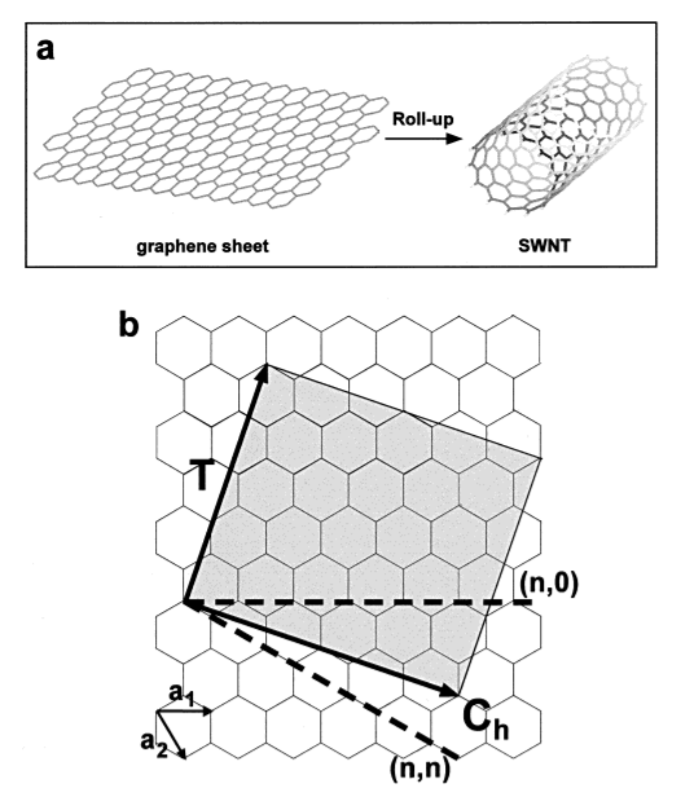
\includegraphics[scale=0.7]{images/chapter_optical_props/chiral_vectors.png}
	\caption{{\color{red}UNFINISHED CAPTION} Reproduced from \cite{odom2000structure}.}
	\label{fig:chiral_vectors}
\end{figure}


\section{Optical Selection Rules}

{\color{red}UNFINISHED} Selection rules dictate the optical transitions that can occur. Such optical processes depend upon the conservation of both energy and angular momentum \cite{weismanKonoBook}. The notation E$_{ij}$ denotes an inter-band transition between the valence sub-band $i$ and the conduction sub-band $j$ \cite{weismanKonoBook}. Incident light polarized parallel to carbon nanotube axial direction excites transitions where $i=j$ \cite{weismanKonoBook}. Incident light polarized perpendicular to the nanotube axial direction can only excite optical transitions where $|i-j|=1$ \cite{weismanKonoBook}. 


\begin{figure}[H]
	\centering
	\begin{subfigure}{\textwidth}
		\centering
		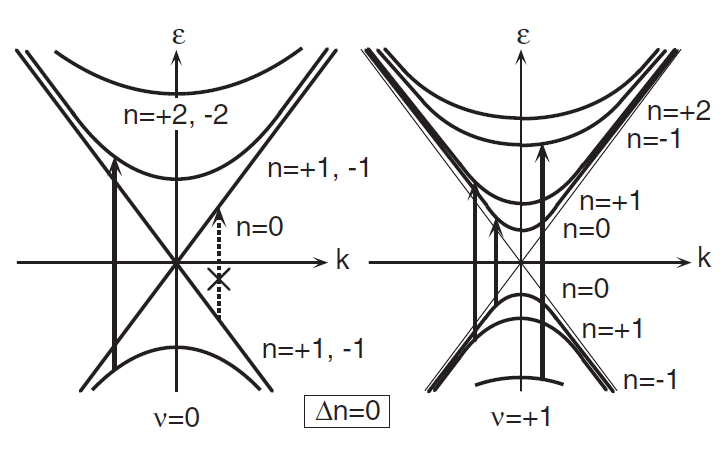
\includegraphics[scale=0.7]{images/chapter_optical_props/selection_rules_1.png}
		\caption{Selection Rules for Parallel case.}
	\end{subfigure}
	\begin{subfigure}{\textwidth}
		\centering
		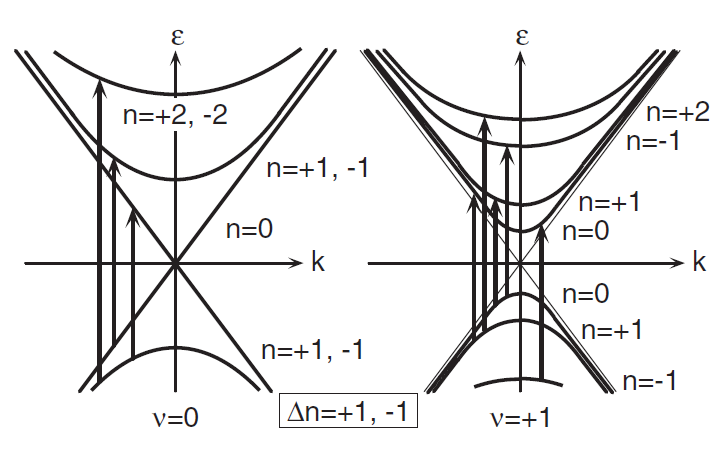
\includegraphics[scale=0.7]{images/chapter_optical_props/selection_rules_2.png}
		\caption{Selection rules for perpendicular case}
	\end{subfigure}
	\caption{Selection rules. Reproduced from Ref \cite{ando2005theory}.}
	\label{fig:selection_rules}
\end{figure}

\section{Excitons in Carbon Nanotubes}

{\color{red}UNFINISHED} In a simple tight-binding picture, density of states consists of Van-Hove singularities in both the valence and conduction bands. This model however ignores the effects of electron-electron interactions. In fact 1-D structures are expected to exhibit stronger quantum confinement than their 2-D and 3-D counterparts, suggesting that electron-electron interactions ought to play a very important role in their electronic structure {\color{red} CITATION NEEDED}. 

\begin{figure}
	\centering
	\begin{subfigure}[t]{0.4\textwidth}
		\centering
		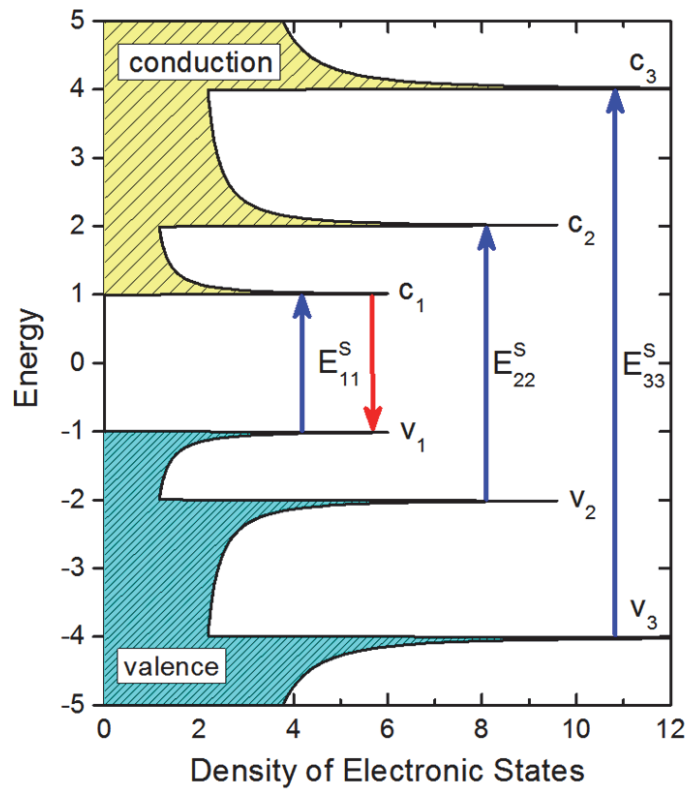
\includegraphics[scale=0.37]{images/chapter_optical_props/dos_semic_weismanKono_book}
		\caption{Semiconducting CNTs}
	\end{subfigure}
	\qquad
	\begin{subfigure}[t]{0.4\textwidth}
		\centering
		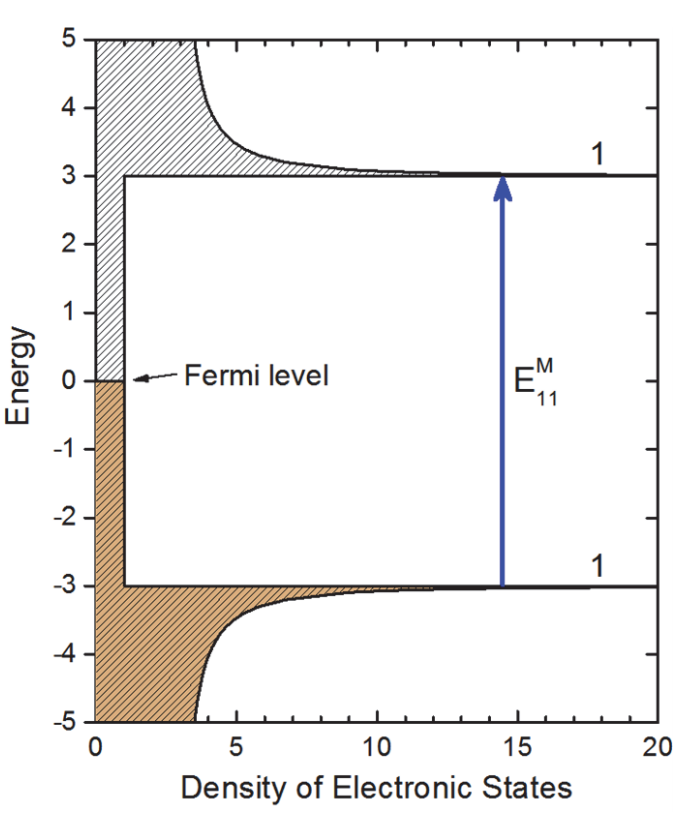
\includegraphics[scale=0.37]{images/chapter_optical_props/dos_metallic_weismanKono_book}
		\caption{Metallic CNTs}
	\end{subfigure}	
	
	\caption{Density of States of semiconducting and metallic nanotubes in a simple tight-binding model. The notations E$_{ij}^S$ and E$_{ij}^M$ indicate inter-band transitions between bands of index $i$ and $j$ for semiconducting and metallic nanotubes respectively.  Reproduced from Ref \cite{weismanKonoBook}.}
\end{figure}

{\color{red}CITATIONS NEEDED FOR THIS PARAGRAPH} Furthermore, these strong electron-electron interactions largely influence the binding energies of quasi-particles known as excitons that form after the creation of an electron-hole pair. Excitons represent hydrogen-like particles composed of a negatively-charged electron bound to a positively-charged hole. Similar to hydrogen atoms, they also possess their own set of analagous optical transitions. In an ideal 1-D material, theory predicts that excitons have an infinite binding energy. This alone foreshadows the dominance of excitons in the optical properties of carbon nanotubes \cite{ando2005theory}. 

Excitonic resonances in carbon nanotubes effectively suppress the oscillator strengths of the free electron continuum states. {\color{red} HOW DOES THIS HAPPEN?}

In fact, all optical excitations in carbon nanotubes lead to the direct creation of excitons \cite{wang2005optical}. How did they show this?

Binding energies on order of hundreds of meV. Means that excitons are quite stable at room temperature. Quite unusual because in contrast, well-known semiconductors such as GaAs only exhibit excitons with binding energies typically less than 10 meV. Samples have to be cooled down to low temperatures in order to easily observe exciton resonances. Unusual dominance of excitons in electronic structure gives opportunity to study physics of excitons. {\color{red} LETS ALSO TALK ABOUT POSITION OF EXCITONIC RESONANCE WRT BAND EDGE}.




\begin{figure}[h]
	\centering
	\includegraphics[scale=0.7]{example-image-a}
	\caption{Figure of GaAs absorbance at low-T and high-T to show weak binding energy of excitons. Next to this is a figure of  (6,5) absorbance at room temperature}
	\label{fig:gaas_vs_cnt_absorbance}
\end{figure}
